\chapter{Implémentation}
        \section{Choix des technologies}
        Au cours de la réalisation d'un logiciel numérique,
        l'une des étapes les plus importantes est de choisir la bonne pile technologique. 
        Pourquoi? Parce qu'il s'agit de créer un produit qui ne consiste pas uniquement
        à concevoir une interface utilisateur agréable et une expérience utilisateur 
        pratique; il s'agit également de concevoir un produit stable, sécurisé et 
        maintenable qui, non seulement est en mesure de charmer les utilisateurs mais encore, vous 
        permettra de faire évoluer l'entreprise.
        \paragraph{}
        Chaque couche de l'application est construite au-dessus d'une autre, 
        formant une pile. Cela rend les technologies Web fortement dépendantes 
        les unes des autres. L'image \ref{fig:pile} montre les principaux éléments constitutifs 
        d'une pile technologique typique; cependant, il peut y avoir d'autres éléments de 
        soutien impliqués.
        \begin{figure}[t]
                \centering
                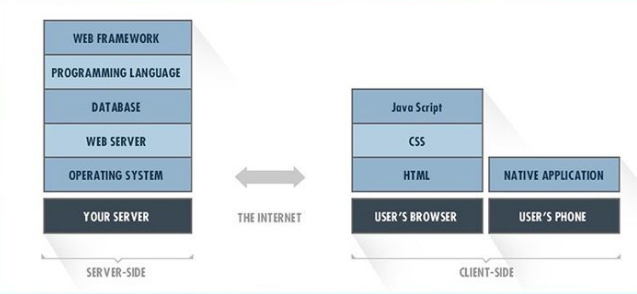
\includegraphics[scale=0.5]{images/Implementation/pile.png}
                \caption{Modèle du cycle de vie en cascade \cite{Bulatovych}}
                \label{fig:pile}
        \end{figure}
        \subsection{Frontend}
        L'interface utilisateur est également appelée côté client, car les utilisateurs voient et interagissent 
        avec cette partie d'une application. Pour une application web, cette interaction s'effectue 
        dans un navigateur web et est possible grâce à de nombreux outils de programmation (Tableau \ref{tab:techoFrontend}). 
        Les applications Web destinées aux clients sont généralement créées à l'aide d'une combinaison 
        de JavaScript, HTML et CSS.
        \paragraph{Outils que nous utilisons pour le développement frontend:}
        \paragraph{HTML: }
        (Hypertext Markup Language) est un langage de programmation utilisé pour décrire 
        la structure des informations présentées sur une page Web. 
        \textit{Le World Wide Web est aujourd'hui l'une des sources d'information les plus 
        importantes. La plupart des données sur le Web sont disponibles sous forme de 
        pages encodées dans des langages de balisage tels que HTML destinés aux 
        navigateurs visuels \cite{yang2003html}.} 
        \par 
        Pour la réalisation de GeoTechMap, nou utilisons HTML5 qui est la cinquième et dernière 
        édition recommandée par le World Wide Web Consortium (W3C) \cite{brooks2010world}.
        \paragraph{CSS: }
         (Cascading Style Sheets) est un langage de feuille de style qui décrit 
        l'apparence et la mise en forme d'un document écrit en HTML. CSS est utilisé 
        pour annoter du texte et incorporer des balises dans des documents électroniques stylisés.
        Le CSS est encore plus important car il doit être pris en compte pour rendre l'applicatgion responsive.
        L'interface utilisateur doit pouvoir s'adapter à n'importe quelle dimention d'écran 
        d'autant plus que nous constatons la montée du trafic web via les téléphones mobiles (Figure \ref{fig:statMobile}).
        \begin{figure}[t]
                \centering
                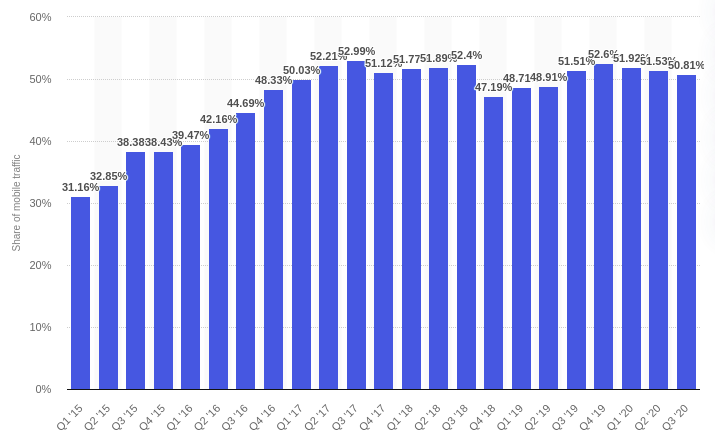
\includegraphics[scale=0.5]{images/Implementation/statMobile.png}
                \caption{
                        Pourcentage du trafic du site Web sur les appareils 
                        mobiles dans le monde du 1er trimestre 2015 au 3ème trimestre 2020 \cite{linkstatmobile}}
                \label{fig:statMobile}
        \end{figure}
        \paragraph{JavaScript (ou JS): }
         C'est la troisième technologie principale pour créer 
        l'interface d'une application Web. JavaScript est couramment utilisé pour créer des 
        pages Web dynamiques et interactives. En d'autres termes, il permet des animations 
        Web simples et complexes, qui contribuent grandement à une expérience utilisateur 
        positive.
        \par
        \textit{JavaScript est devenu le langage de facto pour la programmation Web côté client \cite{gardner2012towards}.}
        \paragraph{React: }
        C'est une bibliothèque JavaScript pour créer des interfaces utilisateur.
        ReactJS offre des solutions élégantes à certains des problèmes les plus 
        persistants de la programmation frontend, vous permettant de créer facilement 
        des applications Web dynamiques et interactives. Il est rapide, évolutif, flexible, 
        puissant et dispose d’une solide communauté de développeurs qui se développe 
        rapidement. \textit{Il s'agit actuellement de la bibliothèque JS frontale la plus populaire \cite{aggarwal2018modern}.}  
        \par    
        \begin{table}
                \centering
                \begin{tabular}{|p{0.30\linewidth}|p{0.10\linewidth}|p{0.60\linewidth}|}
                \hline
                        \textbf{Technologie}&\textbf{Version}&\textbf{Détails}\\
                        \hline
                        HTML&
                        5&
                        HTML5 est conçu pour rendre le développement de ces applications Web 
                        riches plus facile, plus naturel et plus logique, où les développeurs 
                        peuvent concevoir et créer une seule fois, et les déployer n'importe où. 
                        HTML5 rend également les applications Web plus utilisables, car il supprime 
                        le besoin de plugins \cite{wang2013definitive}.
                        \\
                        \hline
                        CSS&
                        3&
                        bla
                        \\
                        \hline
                        JS&
                        ES6&
                        « ES » est l’abréviation d’ECMAScript, le standard sur lequel repose JavaScript.
                        Tous les navigateurs modernes supportent l’ES6 depuis un moment, et les 
                        frameworks majeurs (Angular, React, Vue…) utilisent tous cette nouvelle version de JavaScript
                        \\
                        \hline
                        React&
                        17&
                        \textit{Bien que React v17 ne propose aucune nouvelle fonctionnalité, 
                        il établit une base solide pour les versions à venir en abordant directement 
                        l'expérience de mise à niveau et en alignant plus étroitement le comportement 
                        de React sur les navigateurs modernes \cite{Vardhan2020}.}
                        \\
                        \hline
                      
                \end{tabular}
                \caption{Les technologies utilisées pour le développement du frontend de GeoTechMap} 
                \label{tab:techoFrontend}
        \end{table}
        \par
        \subsection{Backend}
        \subsubsection{Application backend}
        \subsubsection{Base de données}
        \section{La hiérarchie dans l'application}
        \lipsum[1]
        \section{Ergonomie}
        % Interface utilisateur
        \lipsum[1]
        \section{Déploiement}
        \lipsum[1]
        \section{Sécurité du système}
        % -securitaire
        % -high reliability
        % -high scalability
        \lipsum[1]
        \section{Limitations du système}
        \lipsum[1]
        \section{Coûts}
        \lipsum[1]
    
